\documentclass{article}

% if you need to pass options to natbib, use, e.g.:
%     \PassOptionsToPackage{numbers, compress}{natbib}
% before loading neurips_2020

% ready for submission
%\usepackage{neurips_2020}

% to compile a preprint version, e.g., for submission to arXiv, add add the
% [preprint] option:
     \usepackage[preprint]{neurips_2020}

% to compile a camera-ready version, add the [final] option, e.g.:
%    \usepackage[final]{neurips_2020}

% to avoid loading the natbib package, add option nonatbib:
%    \usepackage[nonatbib]{neurips_2020}

\usepackage[utf8]{inputenc} % allow utf-8 input
\usepackage[T1]{fontenc}    % use 8-bit T1 fonts
\usepackage{hyperref}       % hyperlinks
\usepackage{url}            % simple URL typesetting
\usepackage{booktabs}       % professional-quality tables
\usepackage{amsfonts}       % blackboard math symbols
\usepackage{nicefrac}       % compact symbols for 1/2, etc.
\usepackage{microtype}      % microtypography
\usepackage{xcolor}
%Image-related packages
\usepackage{graphicx}
\usepackage{enumitem}
\bibliographystyle{unsrt}

\title{Spatio-Temporal Domain Adaptation for Gait Based User Recognition from Radar Data}

% The \author macro works with any number of authors. There are two commands
% used to separate the names and addresses of multiple authors: \And and \AND.
%
% Using \And between authors leaves it to LaTeX to determine where to break the
% lines. Using \AND forces a line break at that point. So, if LaTeX puts 3 of 4
% authors names on the first line, and the last on the second line, try using
% \AND instead of \And before the third author name.

\author{
  Kalvik Jakkala \\
  Department of Computer Science\\
  University of North Carolina at Charlotte\\
  Charlotte, NC 28223 \\
  \texttt{kjakkala@uncc.edu} \\
  \And
  Chen Chen \\
  Department of Computer Science\\
  University of North Carolina at Charlotte\\
  Charlotte, NC 28223 \\
  \texttt{chen.chen@uncc.edu} \\
  \And
  Minwoo Lee \\
  Department of Computer Science\\
  University of North Carolina at Charlotte\\
  Charlotte, NC 28223 \\
  \texttt{minwoo.lee@uncc.edu} \\
  \And
  Arupjyoti	Bhuyan \\
  Idaho National Laboratory \\
  Idaho Falls, ID 83401 \\
  \texttt{arupjyoti.bhuyan@inl.gov} \\
  \And
  Zhi Sun \\
  Department of Electrical Engineering \\
  University at Buffalo	\\
  Buffalo, NY 14260 \\
  \texttt{zhisun@buffalo.edu} \\
  \And
  Pu Wang \\
  Department of Computer Science\\
  University of North Carolina at Charlotte\\
  Charlotte, NC 28223 \\
  \texttt{pu.wang@uncc.edu} \\
}

\begin{document}

\maketitle

\begin{abstract}
Radar-based biometric identification is an emerging user identification platform that exploits radar return signals to capture human biometrics (such as gait, gesture, lip motion, and cardiac motion), which can be used to predict a user's identity. Despite its unique advantages (such as privacy-preserving and resilience to weather/lighting conditions), the generalization performance of this technology is still unknown and greatly hinders its practical deployment. To address this challenge, we collect and investigate a non-synthetic dataset, which revealed the existence of distinct spatial and temporal domain shifts in radar-based gait biometric data. We show that spatio-temporal domain shifts, when not addressed jointly, can significantly degrade identification accuracy. Moreover, we propose a data-efficient yet straightforward domain shift mitigation approach for tuning deep learning models over their entire life cycle. Our approach exploits an unsupervised domain shift detector to measure the malignancy of domain shifts. Such metrics allow us to determine the domains that maximize the net contributions upon adapting to, after which an appropriate domain adaption method is utilized to improve both spatial and temporal generalization. We show that our approach improves data efficiency by reducing the number of domains that necessitate adaptation while maintaining the generalization performance of a blind approach that uses data from all domains.
\end{abstract}


\section{Introduction}
\label{intro}
As an emerging user identification technology, radar-based biometric identification exploits radar signals scattered and returned by human subjects to capture a variety of behavioral and physiological biometrics such as gait \cite{wifigait1,pokkunuru2018neuralwave, jakkala2019deep, janakaraj2019star, pegoraro2020multi, huang2020multi, lang2019person, abdulatif2018study, qiao2020human, lang2019joint}, gesture \cite{gesture1,gesture2}, lip motion \cite{lip1,lip2}, and cardiac motion \cite{heart1,heart2}. These biometrics characterize the movement patterns unique to each individual. Radar-based biometric identification systems have several unique advantages. First, they are privacy-preserving as they do not rely on images of human subjects. Next, they can operate in adverse weather and lighting conditions such as heavy fog, smoke, rain, and zero-light conditions. Finally, they can see through some opaque objects depending on its material and the frequency of the radar \cite{wall1,wall2}.

A rich body of research has established the viability of this new technology \cite{wifigait1,pokkunuru2018neuralwave, jakkala2019deep, janakaraj2019star, pegoraro2020multi, huang2020multi, lang2019person, abdulatif2018study, qiao2020human, lang2019joint,gesture1,gesture2,lip1,lip2,heart1,heart2}. However, the spatial and temporal generalization performance of this technology is still unknown. We found that deep neural networks (DNNs) trained on radar-based gait data suffer from substantial performance degradation with the progression of time and in new locations. Most radar-based biometric systems proposed in the literature, test their performance on a dataset collected alongside the training data and fail to uncover the temporal degradation. Furthermore, they seldom address the spatial generalization issues from introducing new environments. These issues are prevalent in other biometric solutions, such as images as well. Nevertheless, curating a dataset of monumental proportions often overcomes this, which is especially true for face recognition, as they have datasets containing millions of images. A brute force approach is not viable for most of the other biometric identification platforms, such as radar-based ones. Unlike images, most other platforms require specialized devices that are not omnipresent and exclusively designed for user recognition, which further complicates data collection campaigns on a large scale.

The root cause of this generalization issue is dataset shift \cite{moreno2012unifying}. Simply put, it occurs when the testing data distribution differs from that of the training data, i.e., the i.i.d. assumption is violated. Depending on the type of difference in the test data distribution, it can be categorized as a covariate, posterior probability, or concept shift. Mitigating dataset shift, also known as dataset drift or domain shift, is known to be one of the hardest problems in machine learning and is prevalent in numerous application domains. This leads us to the ethos of Domain Adaptation, addressed by myriads of methods in literature \cite{wang2018deep}.

After an in-depth analysis of dataset shifts and domain adaptation, we found the current taxonomy of domain shifts is not adequate to explain the full extent of our problem. Apart from the manifestations of domain shifts mentioned above, we seek to distinguish them further. Concretely, we acknowledge the presence of spatial and temporal domain shifts (SDS/TDS). We treat TDS as shifts that arise temporally as a consequence of the inherent dynamics of a domain while, treating SDS as shifts induced from introducing new spatial locations. This distinction allows us to understand and explain the behavior of the shifts that manifest in radar-based gait data.

Before addressing a shift, we need to be aware of its presence. An overwhelming amount of domain adaptation methods only address shifts that behave similar to SDS \cite{wang2018deep}, i.e., they only consider explicitly introduced domains. So, the problem of detecting the presence of a shift, which is a sine qua non for TDS, has not received the attention it deserves. Moreover, among the work available on drift detection \cite{rabanser2019failing}, a majority of them make assumptions about the behavior of softmax classifiers, which have long been invalidated \cite{gal2016dropout, snoek2019can}. We draw attention to a simple yet effective unsupervised domain shift detector based on metric learning \cite{kaya2019deep}.  Our shift detector enables a data-efficient domain shift mitigation approach, where the shift malignancy of each domain is first measured, and domains that maximize the net contributions upon adapting are selected. An appropriate domain adaption method is then applied only to the selected domains to improve model generalization. Our prominent contributions and findings are as follows.
\begin{itemize}[leftmargin=*]
  \item We curated a non-synthetic dataset consisting of radar-based gait biometric data. This dataset, for the first time, allows one to study and improve the spatio-temporal generalization performance of a radar-based biometric identification system.
  \item We introduced the distinction of TDS and SDS, which enables us to explain the system performance degradation. 
  \item We uncovered a correlation between TDS and SDS, which unveiled significant ramifications for data collection and domain adaptation. In particular, we found SDS can be mitigated to a certain extent by using the TD data and vice-versa, but both SDS and TDS have to be addressed explicitly for consistent generalization performance.    
  \item We revealed that if multiple sources of domain shifts appear, each source of domain shifts yields a different net contribution to generalization upon adapting to that domain.
  \item We elucidated the effectiveness of metric learning based shift detectors and reaffirm the limitations of softmax thresholding for out of domain detection. 
  \item Finally, we exploit our shift detector to develop a data-efficient domain shift mitigation approach.
\end{itemize}

\section{Dataset}

\begin{figure}[ht]
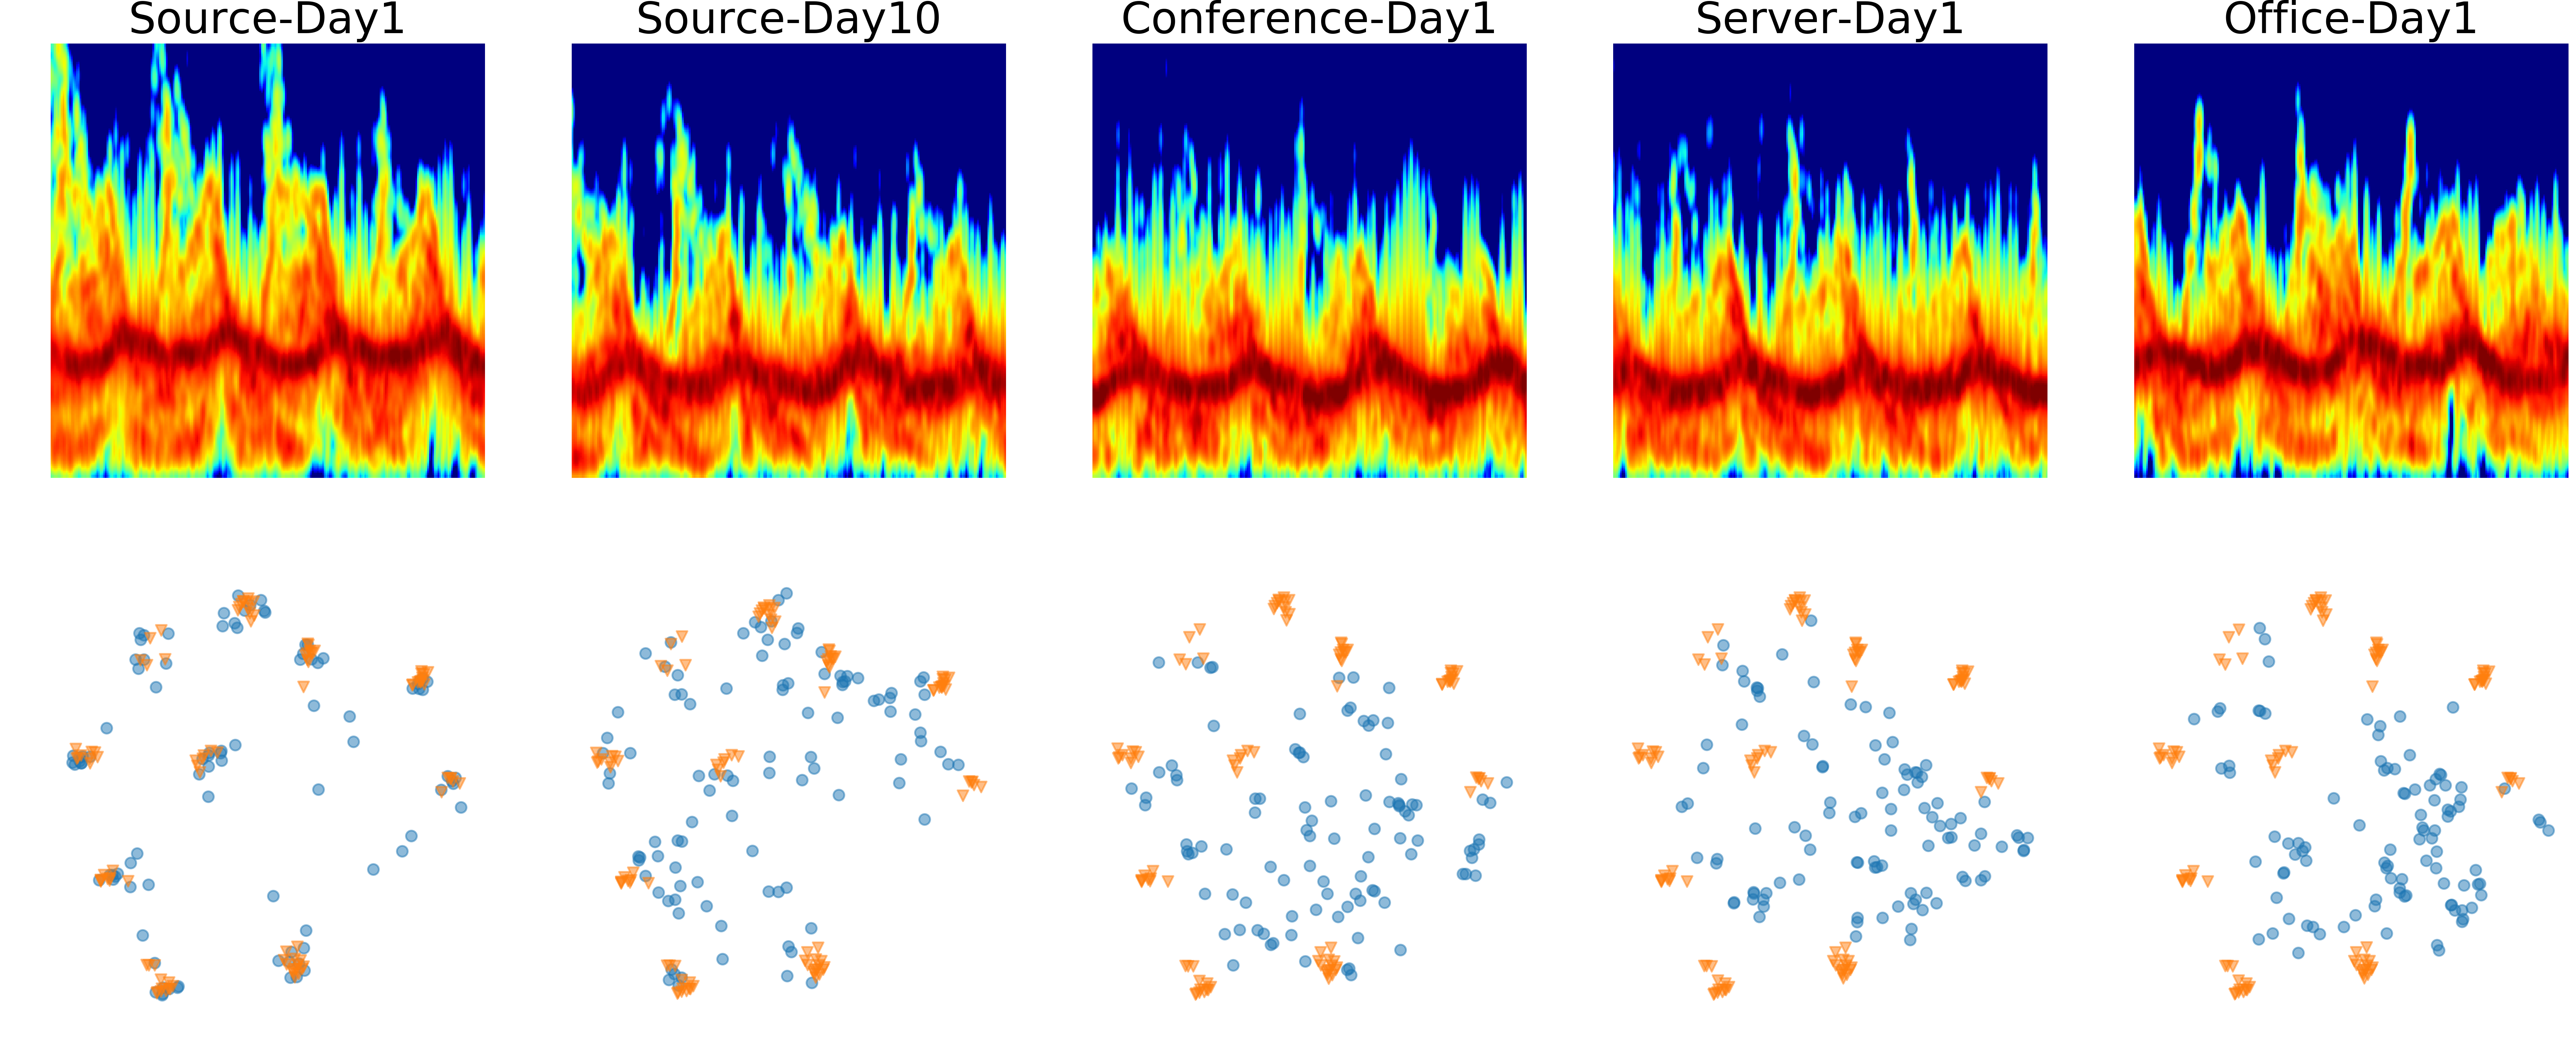
\includegraphics[width=1.0\linewidth]{figures/Exp0.png} 
\caption{First row: gait spectrograms of the same person. Second row: t-SNE embeddings generated from each domain of our dataset. Orange triangle clusters represent the training data in source location on day 1, where each cluster represents a distinct human subject. Blue circles represent each domain's testing data, where the data points were sampled from all the classes of a given domain.}
\label{specs}
\end{figure}

In light of the novelty of our problem, we curated a dataset to study it properly. We collected gait data from 10 volunteers between the ages of 18-35. Each subject's data was collected in four different locations. The source location was a research space with cubicles, and the other three areas consisted of a server, conference, and an office room. By maintaining four distinct locations, we introduce SDS. In the source location, data was collected on ten different days for each subject. Five separate days of data was acquired for each of the three other locations, which are used as target domains.

The data collection was limited to 100 data samples in the source location and 50 data samples in each of the target locations on any given day.  Unlike cameras, radars collect data actively by broadcasting signals into the environments. Unique movement patterns (e.g., gait) can induce different micro-Doppler frequency shifts in radar return signals, which can be represented as a spectrogram. Thus, a radar spectrogram can serve as the biometric print for user identification \cite{wifigait1,pokkunuru2018neuralwave, jakkala2019deep, janakaraj2019star, pegoraro2020multi, huang2020multi, lang2019person, abdulatif2018study, qiao2020human, lang2019joint}. Apart from biometric traits, radar spectrogram data could also contain spatio-temporally varying noises from signal reflections and interference, which cannot be completely removed. This leads to environment-induced TDS and SDS. To add on, human gait, although unique to each individual, could contain minute variations, potentially as a consequence of a subject's mood, clothing, footwear, or some other similar aspect, which combined with the environment-induced shifts, further aggravates TDS. Changing the number of days in the train and test sets changes the amount of TDS. Similarly, using a subset of the available locations, SDS can be controlled, which makes it possible to study how the two variants of shifts interact with each other. 

We use the widely-adopted radar data preprocessing schemes to minimize environment-induced shifts \cite{wifigait1,janakaraj2019star,pegoraro2020multi}\footnote{Refer to the supplementary material for additional details}. It is worth to note in Fig.~\ref{specs} that the spectrograms from all locations look very similar. This is because they are spectrograms representing the same action (gait). Most of the environmental data is filtered out by the preprocessing methods, but the minuscule amounts of environmental information that seeps through was enough to induce domain shifts. We show the t-SNE \cite{maaten2008visualizing} embeddings for each domain in our dataset alongside the training data embeddings. The model used to generate the embeddings was trained on a single day's data from the source location. The embeddings show a domain shift in each new domain. However, this might not be very evident in the absence of the knowledge of the data collection procedure. We address this issue in Section.~\ref{shift}.

\section{Method}
\label{method}

\begin{figure}[ht]
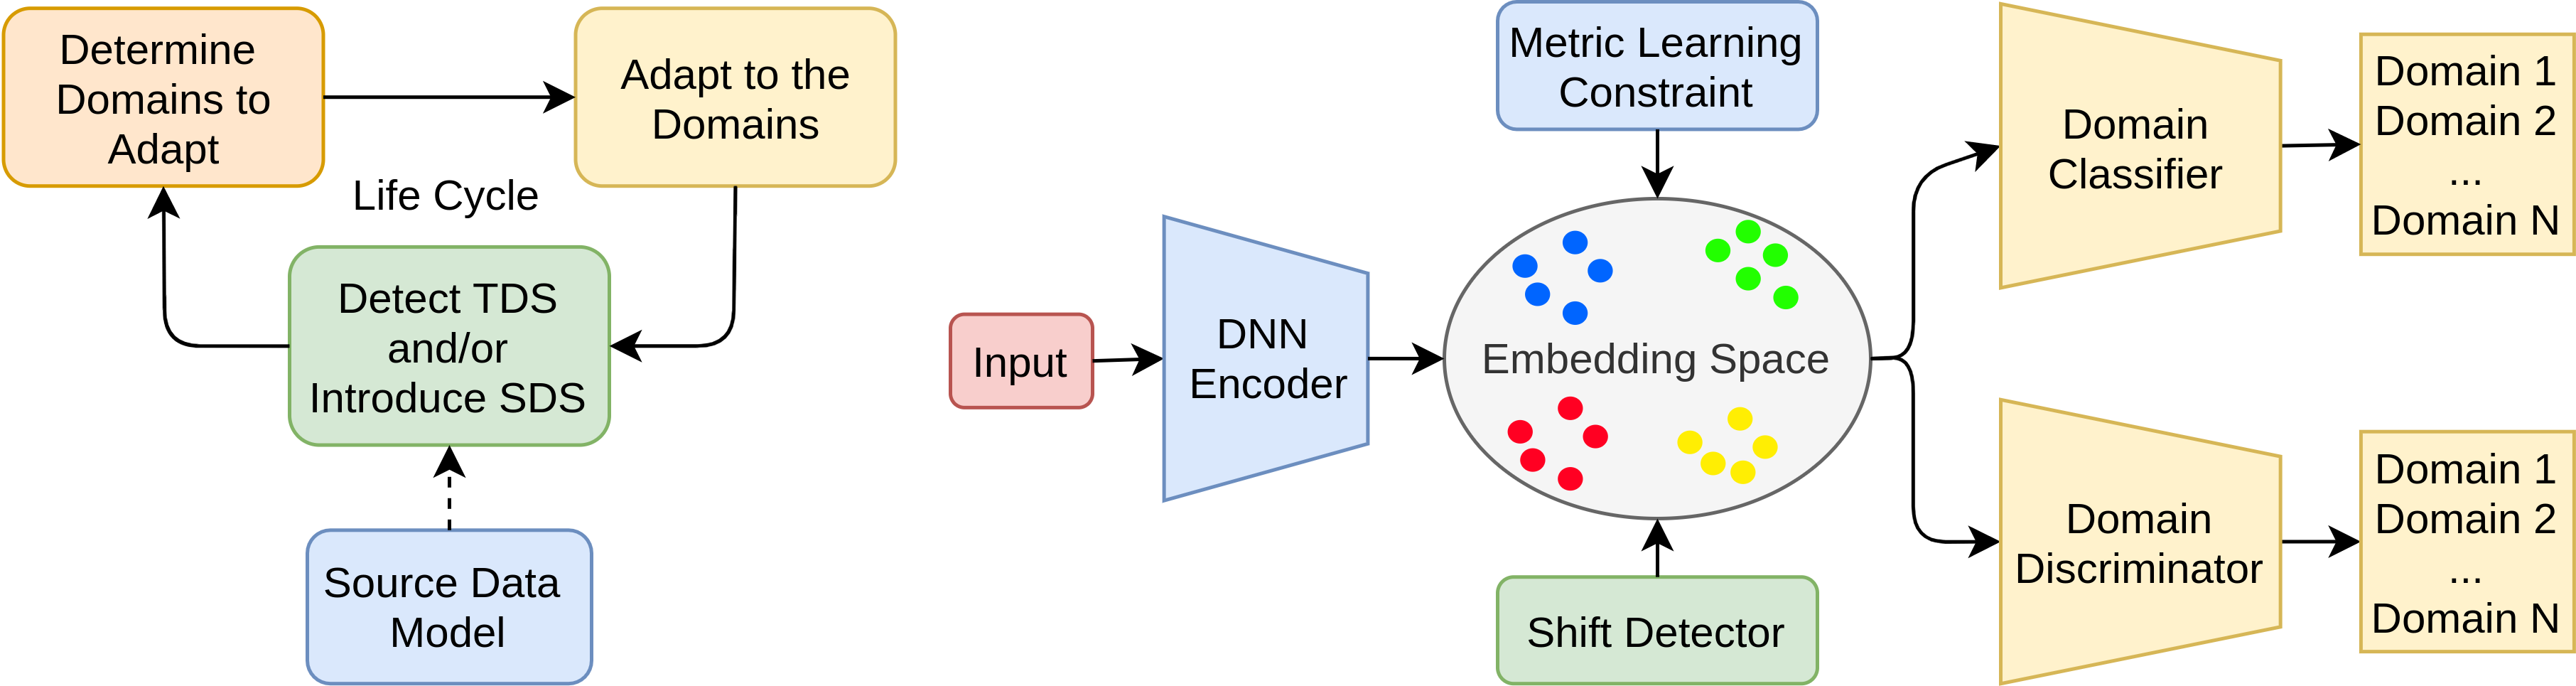
\includegraphics[width=1.0\linewidth]{figures/Arch.png} 
\caption{Left: high-level procedure overview. Right: detailed system model}
\label{arch}
\end{figure}

\textbf{Overall Domain Shift Mitigation Procedure.} Given the radar data in the source location, we utilize metric learning to detect the presence of any TDS and SDS and measure the shift malignancy. Using these metrics, we determine the domains that mandate domain adaptation and ignore the rest. Then, labeled or unlabeled data from the corresponding domains is collected, and an appropriate domain adaptation method is applied. The entire procedure shown in Fig.~\ref{arch} is repeated throughout the life cycle of the deployed model. We explain each component of the proposed procedure as follows.

\textbf{Metric Learning for the Base Model.} Given the user recognition task at the core of our dataset, we started with a metric learning-based model \cite{kaya2019deep}. Training networks with metric learning allows one to introduce new classes after training a base model, without having to train the model again, which translates to adding new user identities without the need for retraining. Another benefit of using metric learning is its theoretical underpinning, which is the cluster assumption. The cluster assumption states that the decision margins lie in low density or relatively unoccupied regions of the classification manifold. This assumption has previously been exploited in numerous domain adaptation techniques and is known to promote adaptation under certain constraints. Metric learning reaffirms this assumption by maximizing inter-class distances and minimizing intra-class distances.

\textbf{Shift and Malignancy Detection.} Upon further investigation, we found metric learning-based models are well suited for detecting domain shifts as well. Domain shift detection is the process of identifying shifts in the testing data. Unlike SDS, the presence of TDS is not always known. A few methods have been proposed for domain shift detection, but most either fail to detect shifts in an online fashion \cite{lipton2018detecting, rabanser2019failing} or base their predictions on softmax thresholding. However, it is well established that \cite{gal2016dropout, snoek2019can} softmax classifiers are not suitable for detecting domain shifts, especially for out of domain data. 

To address aforementioned challenge, we rely on thresholding embeddings generated by metric learning models. Softmax classifiers are optimized to make closed-set predictions \cite{geng2020recent}, i.e., pick one of the classes present in the training dataset as the prediction. Such an assumption is too strong and grossly underestimates the likelihood of seeing unknown classes or out of distribution data during testing. Metric learning methods do not make such assumptions or, at the very least, not to the extent softmax based solutions do. Metric learning optimizes a metric on embeddings generated by a base classifier, which potentially allows the classifier to ignore the concept of closed set predictions, thereby overcoming overconfident predictions and calibration issues.

We exploit this premise to detect domain shifts. By maintaining dictionaries of class-wise mean embeddings and thresholding any new data point's distance from known embeddings, we can recognize shifts and their magnitude. Furthermore, such an approach does not require any specific offline training and can be deployed on online data sources. Not to mention, the detector will also be unsupervised, as no labeled data is required to detect a shift. The notion of detecting outliers or novel classes from embeddings is certainly not unheard of. We re-purpose it for detecting the presence and extent of domain shifts. Our experiments show that the approach agrees with labeled shift detectors. 

\textbf{Data-efficient Domain Shift Mitigation.} Exploiting the proposed domain shift detector enables us to develop a data-efficient domain shift mitigation approach. Instead of blindly collecting a large amount of labeled or unlabeled data from all spatial and temporal domains, we use the shift detector to measure the shift malignancy of each domain. Next, domains with insignificant shifts are discarded. Based on the cost of collecting labeled/unlabelled TD/SD data in different domains, a heuristic approach is utilized to determine and collect an appropriate type and amount of data. After this, the available domains are adapted to using an appropriate domain adaption strategy. A hybrid domain adaption scheme can also be applied, where supervised domain adaption is used to address certain shifts and unsupervised methods for the others.

For unsupervised domain adaptation, we experimented with three prominent methods. In the first method, we combine metric learning and a domain discriminator based on a gradient reversal layer (GRL) \cite{ganin2016domain}. As anticipated, the approach worked well. The addition of metric learning boosted the model performance by a sizable amount. In the second approach, we replace the GRL with a Generative Adversarial Network \cite{goodfellow2014generative}, which can also significantly improve model generalization performance (which is detailed in section 4.6). Finally, we used a student-teacher based approach \cite{meng2018adversarial} but failed to procure any significant improvement. We conjecture that the failure is due to the presence of metric learning. The recent findings of  \cite{muller2019does} have a strong resemblance to combining student-teacher with metric learning. Since label smoothing behaves similar to metric learning, we speculate the presence of metric learning impedes the need for student-teacher approaches.

\section{Experiments}
All of our experiments utilized an 18-layer Resnet architecture \cite{he2016deep}. The models were trained using an Adam optimizer \cite{kingma2014adam} with an initial learning rate of 1e$^{-3}$ and polynomial decay\footnotemark[\value{footnote}]. Additionally, we used Constrictive Annular Loss (CA-Loss) \cite{liu2019learning} for metric learning. It is a regularised variant of Additive Margin Softmax  \cite{wang2018additive}. Nevertheless, we speculate that any metric learning based approach could be used in place of CA-Loss to draw similar conclusions as we do here.

\subsection{Establishing the Presence of TDS and SDS}
\label{pres}

\begin{figure}[ht]
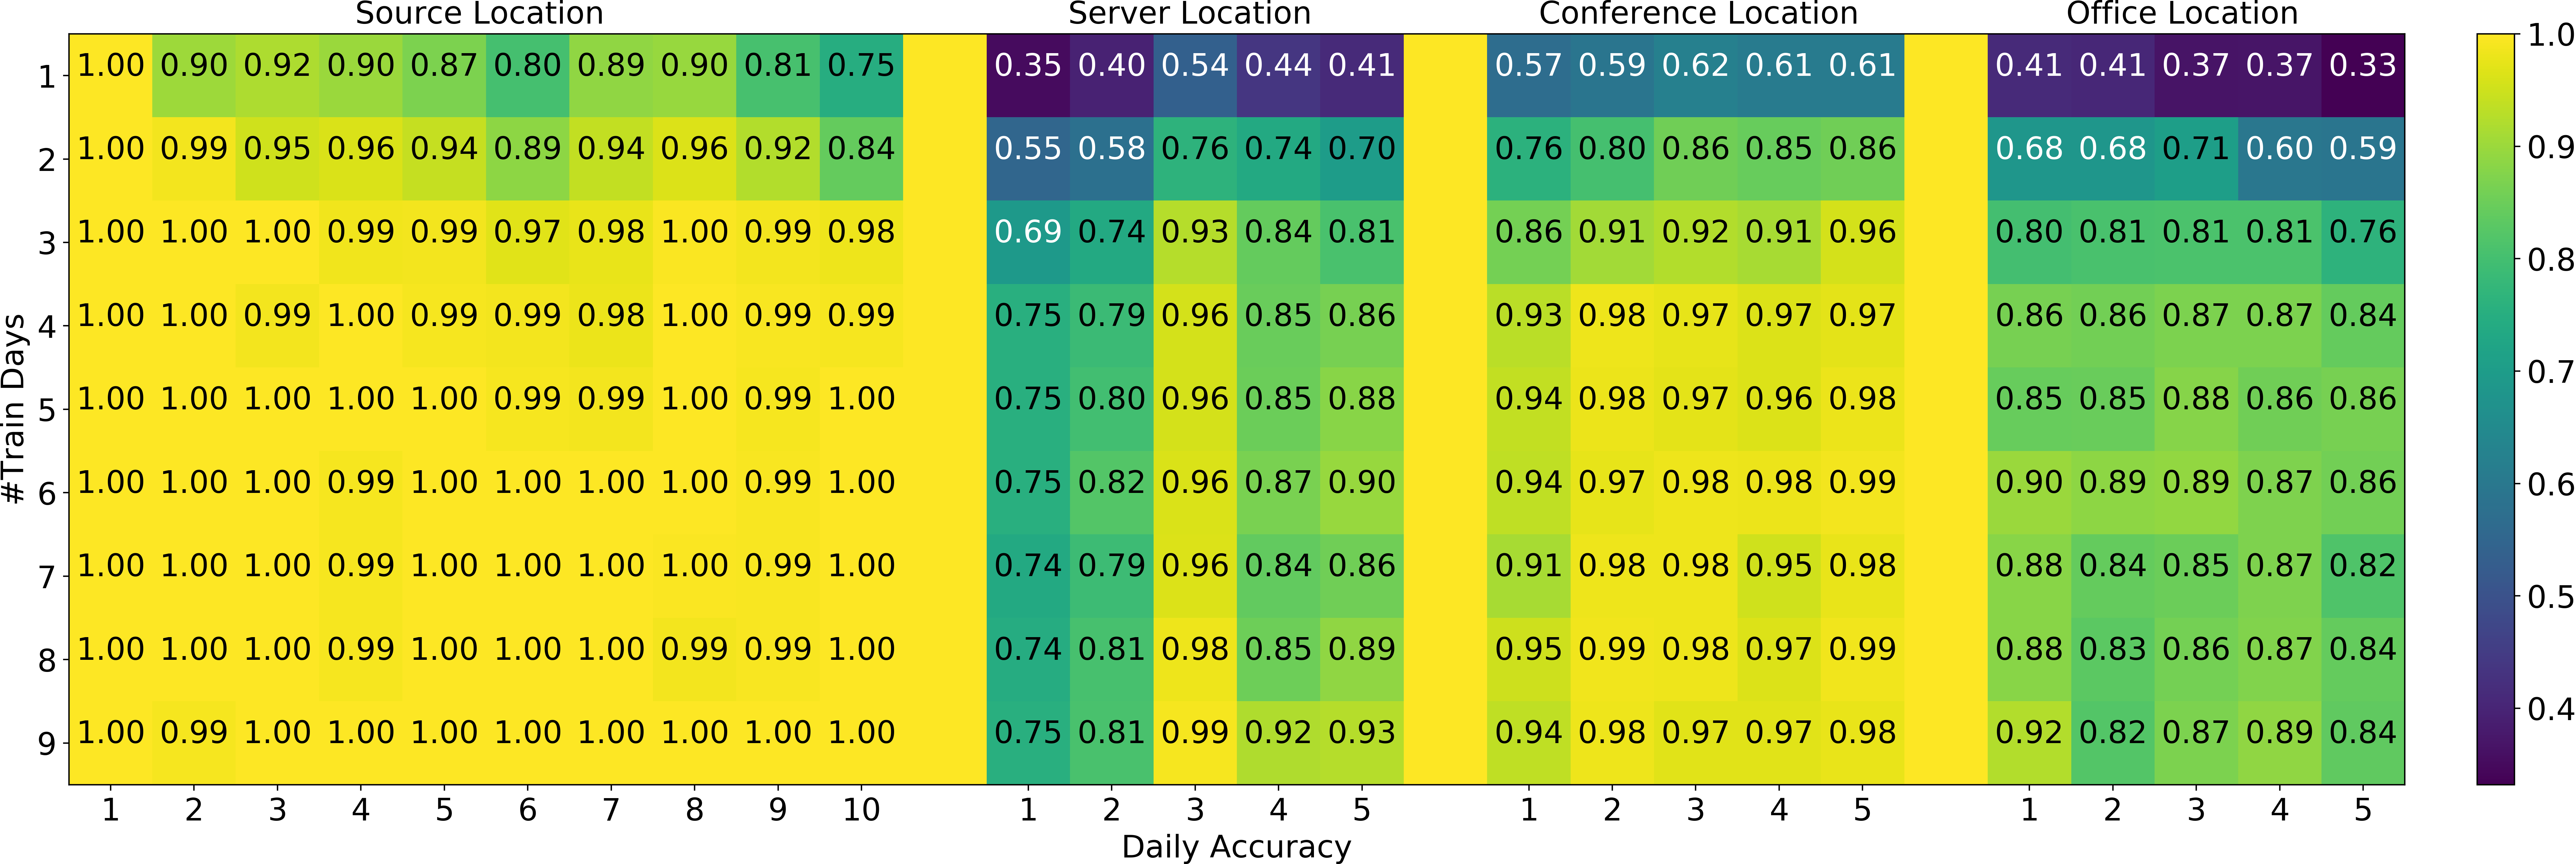
\includegraphics[width=1\linewidth]{figures/Exp1.png} 
\caption{Results obtained from training only on source location data for varying number of days.}
\label{src}
\end{figure}

Our first experiment establishes the presence of TDS and SDS in our dataset. We trained a model on data only from the first day of our source location. Test accuracies of data from the remaining nine days of the source location and all target locations are reported in Fig.~\ref{src}. The temporal degradation in the source and target domains is evident in the \emph{first row} of Fig.~\ref{src}. 

The target domains also suffer from SDS apart from TDS, which is evident from the overall performance degradation in the target domains. This unequivocally establishes the presence of both TDS and SDS in our dataset. We also found a rather unexpected outcome from this experiment. There is a temporal degradation both in the source and target locations, but the deterioration does not strictly correlate with time progression. We conjecture that this behavior is a consequence of the malignancy of shifts. That is, not every shift is equally harmful. We further elaborate on this in Section~\ref{dom_imp}.

\subsection{Mitigating TDS and SDS}
\textbf{Mitigating SDS via TD data.} We now show that it is not possible to entirely mitigate SDS by introducing source domain's temporal data alone and vice-versa. Limitations of improving SDS generalization by using TD data are evident in Fig.~\ref{src}. We trained models from two, all the way up to nine days of labeled source location data, which is followed by an evaluation of daily accuracies. By introducing more temporal data, the source location generalization improves as time progresses. But as one might expect, we start to see diminishing returns in terms of source location accuracy as we increase the number of training days. Moreover, after introducing more source domain's temporal data, the target location performance also has diminishing returns so that each target location's performance is seldom on par with the source. 

\begin{figure}[ht]
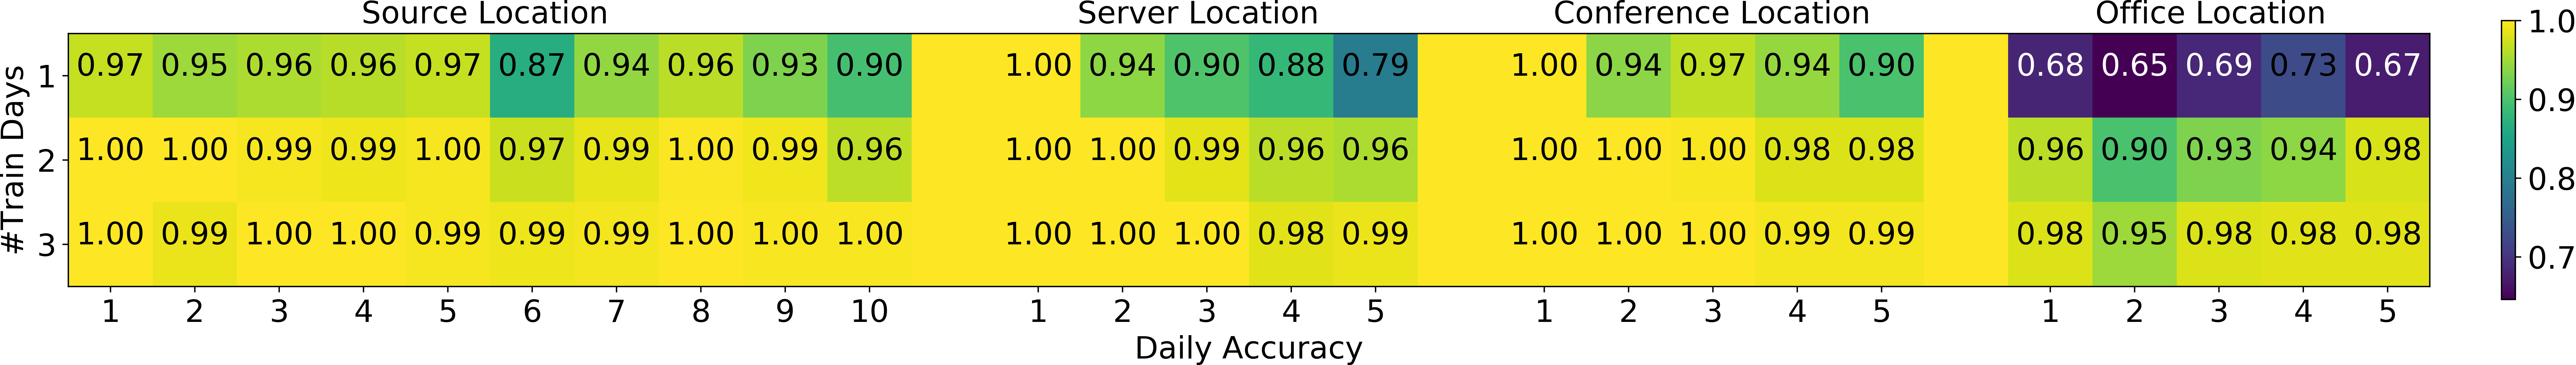
\includegraphics[width=1.0\linewidth]{figures/Exp2.png} 
\caption{Results obtained from training on source, server, and conference location data for varying number of days. The data from office location is not used for training and only for testing}
\label{trg}
\end{figure}

\textbf{Mitigating TDS via SD data.}  We move on to establish the limitation of introducing more target/spatial domain data to alleviate TDS. We trained a model on a single day of labeled data from the source, conference, and server locations. From the \emph{first row} of Fig.~\ref{trg}, it is clear that even when data from target domains is introduced, individual location's temporal shifts are not completely mitigated. However, we do find that the model performance in the office location improves when compared to introducing only temporal data. Since no data from the office was used in training, we interpret it as the true SDS generalization of the model. This implies that the primary benefits of training on data from a particular type of shift is confined to easing similar kinds of shifts. 

\subsection{Correlation of TDS and SDS}
We now draw attention to the correlation between TDS and SDS. It is evident from our prior experiments that TD or SD data individually cannot mitigate both. Nevertheless, from Fig.~\ref{src} and Fig.~\ref{trg}, and the findings mentioned above, a correlation between the two is evident. It might be the reason no clear distinction has been established so far, but the implication of this is rather profound. Collecting TD and SD data might incur varying costs. \emph{When the cost disparity is substantial, it is possible to trade one for the other to a certain extent}. This brings us to one of the most exciting findings of our paper. That is, \emph{TDS and SDS have to be addressed jointly to bring substantial generalization improvement}. We trained models with both TD and SD data along with the initial source data. We find in Fig.~\ref{trg} that when both shifts are addressed together, we attain the best generalization in both TD and SD. By introducing multiple (2 - 3) days of data from every location, we address TDS individually in each location. Introducing data from multiple target locations (server and conference rooms) addresses SDS. Moreover, such jointly trained model generalizes well to the unseen target domain (office).

\subsection{Domain Importance}
\label{dom_imp}

As mentioned in Section~\ref{pres}, we notice a disparity in the malignancy of each domain shift. From the plethora of research conducted on adversarial learning \cite{chakraborty2018adversarial}, it is evident that not every kind of data noise is equally harmful. Networks can overcome small amounts of noise in the data. This is true even when the models have not been explicitly trained with adversarial methods. Similarly, adversarial training with arbitrary data perturbations is not always a precursor for domain generalization. 

\begin{figure}[ht]
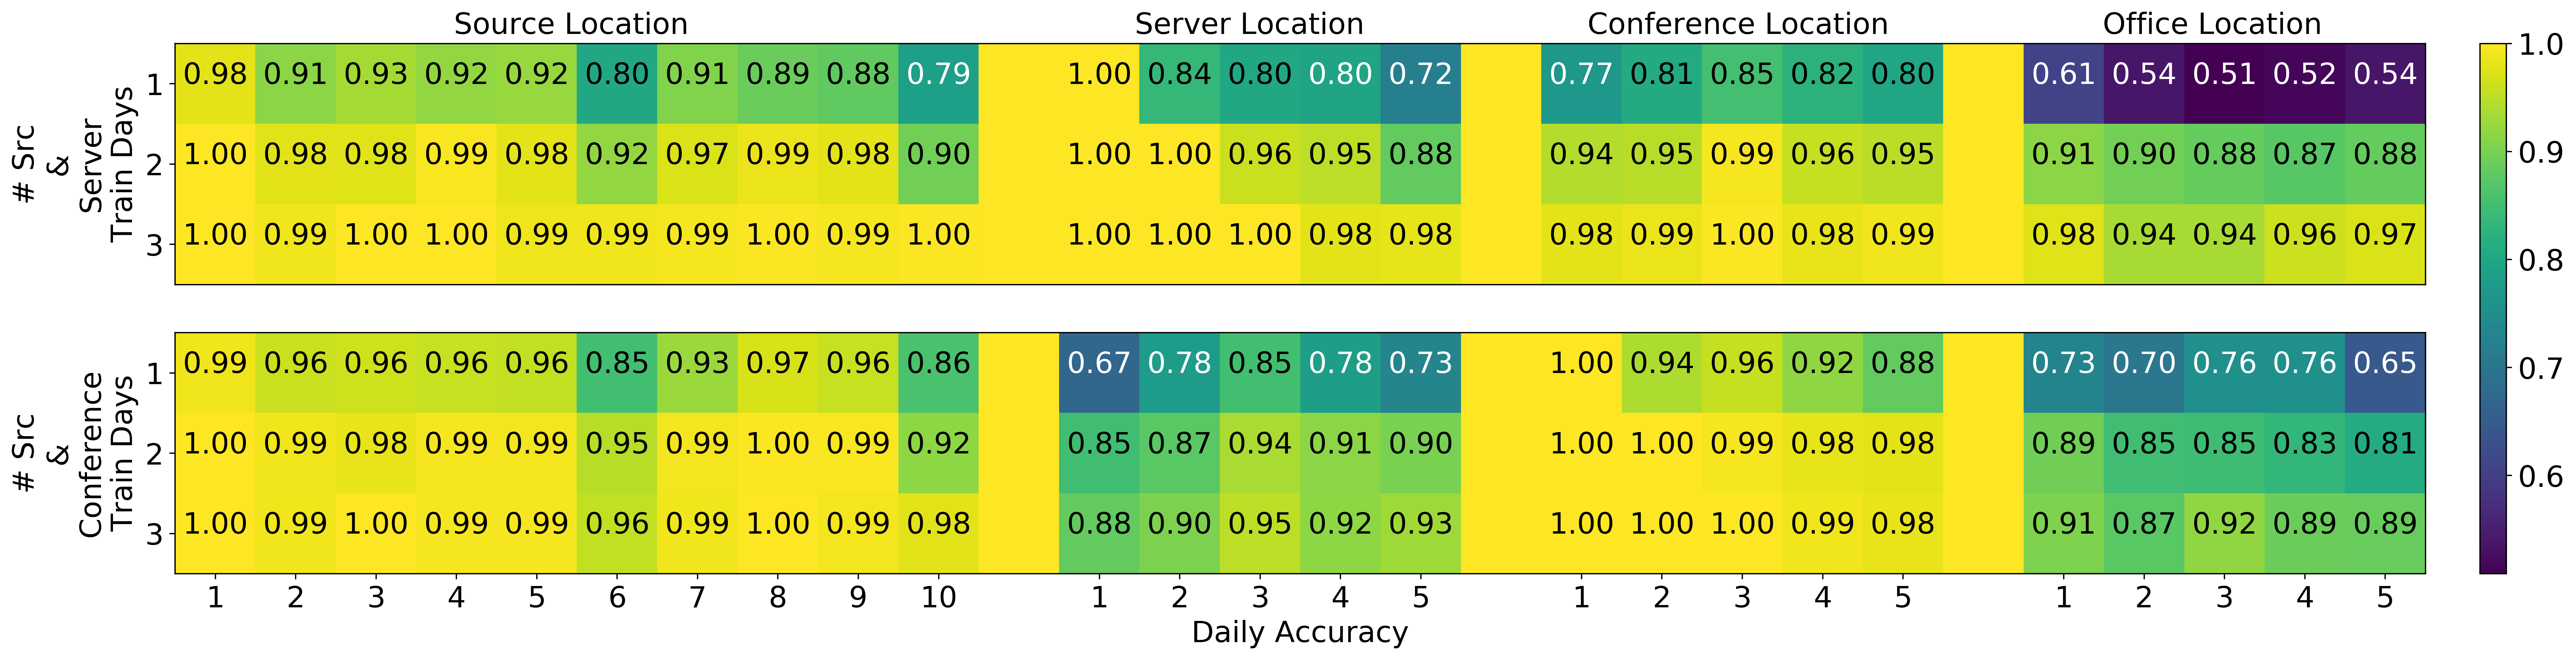
\includegraphics[width=1.0\linewidth]{figures/Exp5.png} 
\caption{(Top) Results obtained from training on the source and server data for a varying number of days. (Bottom) Results obtained from training on the source and conference data for a varying number of days. Data from office location is for testing only}
\label{exp5}
\end{figure}

We find this to be the case for domain adaptation as well. Not all available domains are worth adapting to. In our dataset, the conference location exhibits a domain shift, but it is not equally worth adapting to when compared to server room data. We found that by adapting to the server location alone, we can generalize to all other locations shown in Fig.~\ref{exp5}. The server room can be considered more adversarial than the conference room. When we train a model on the source and server data, the information discrepancy amongst the two domains is substantial compared to the source and conference room data. This results in spatial generalization with only half of the spatial target domain data. Admittedly, the model trained with source and server data is not as good as the model trained with source and conference data in every aspect. However, the overall generalization is better. Depending on the cost of data collection, it might be well worth the marginal loss in accuracy. This raises the question of how one can estimate the potential gains in generalization upon adapting to a domain, and we address this issue in Section~\ref{shift}.

\subsection{Shift Detection}
\label{shift}

\begin{figure}[ht]
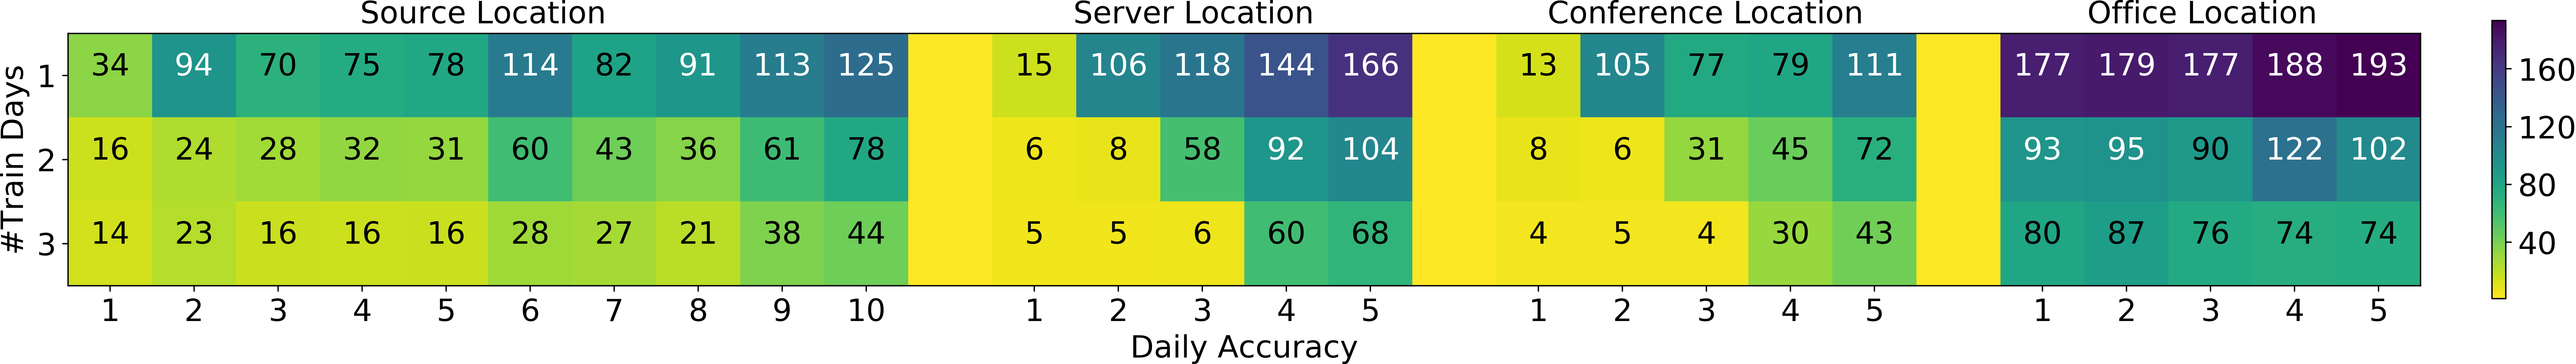
\includegraphics[width=1.0\linewidth]{figures/Exp4.png} 
\caption{Mean distance from known class centers obtained from the source, server, and conference data for a varying number of days.}
\label{exp4}
\end{figure}

As mentioned in Section~\ref{method}, before addressing domain shifts, we must be aware of the existence of a shift in their data. So far, we used an offline approach for shift detection, where the accuracy of the model trained using ground truth labels is used to uncover the presence of domain shifts. We now propose to sidestep this issue. By thresholding the distance to known training data embeddings, we acquire results similar to our labeled, accuracy based observations. Not only does this need no ground truth labels, but it can also be deployed online without any specific training for the problem. We note that a separate holdout dataset will be required to tune the thresholds\footnote{Refer to the supplementary material for additional details}. An added advantage of such an approach is its capability of detecting the malignancy of a shift. The accuracy-based approach does not necessarily convey the amount of shift introduced \cite{gal2016dropout, snoek2019can}. We amend this issue by interpreting the magnitudes of the distance from class centers as an indicator of its malignancy. In Fig.~\ref{exp4}, we present the results of Fig.~\ref{trg}, but with metric learning based shift metrics\footnote{Refer to the supplementary material for metric learning based results of all our experiments along with t-SNE embeddings, and elaboration of additional findings from the magnitude of shifts.}. We find that the results strongly correlate with our hypothesis along with insights\footnotemark[\value{footnote}] into the malignancy of each domain. 

\subsection{Data-efficient Domain Shift Mitigation}

\begin{table}[ht]
\caption{Model Accuracies (\%). (Labeled) The model trained on three days of labeled source, server, and conference data. (Hybrid) The model trained on three days of labeled source data and three days of unlabeled server data.}
\begin{center}
\begin{tabular}{ccccc} 
\hline
  & Source-Temporal & Server-Test & Conference-Test  & Office-Test \\
\hline
 Labeled & 99.59 & 98.85 & 99.37 & 97.51 \\ 
\hline
 Hybrid(Ours) & 99.61 & 98.70 & 99.70 & 97.47 \\ 
\hline
\label{uda}
\end{tabular}
\end{center}
\end{table}

All the experiments we reported so far were exclusively trained with labeled data. Nevertheless, that need not be the case. We utilized a domain discriminator trained as a GAN\footnotemark[2] to adapt to TDS and SDS. We trained a network with three days of labeled source location data and three days of unlabeled server location data, which makes TDS adaptation in the source domain supervised. However, TDS and SDS adaptation in the target domains is addressed in an unsupervised manner. Table~\ref{uda} shows the results of our approach (Hybrid) and results from training a model without a discriminator on three days of labeled source, conference, and server data. We reduced the amount of labeled data by utilizing unsupervised domain adaptation techniques. Furthermore, utilizing the lessons learned from our findings so far, the number of domains to adapt was reduced, i.e., we only use the server location data with the highest domain shifts, while ignoring data from conference and office locations. Furthermore, we conjecture that by incorporating few-shot learning methods, the source location labeled data could also be reduced. A single day of source location data currently consists of only 1000 labeled data samples, which hinders the performance as it is not sufficient to train a robust model. We addressed this issue by using labeled data from three days of the source location. However, using other techniques such as initialization with pre-trained model weights might also work well, thereby reducing the source location's labeled data.

\section{Discussion}
With all our experiments and findings being detailed, we now move on to discussing their implications. 

\textbf{Detecting Shifts.} The first and foremost question is to detect shifts. By incorporating metric learning, one can detect shifts with thresholding. Merely being aware of the proper tools to detect a shift will be a great take away from our work. Since softmax based methods are invalid,  our method is a straightforward alternative. However, a thorough investigation into how accurate these metrics are on a wider variety of datasets, with longer time horizons, is needed. 

\textbf{Handling Shifts.} Upon detecting a shift, the question of how to handle it naturally arises, which entails figuring out how much and which data should be acquired. As mentioned in Section~\ref{dom_imp}, we suggest one should take account of the malignancy and the type of shift in such decisions. Being aware of the malignancy of every shift allows one to determine which domains need to be adapted to, thereby significantly reducing any resources involved in the adaptation process. Shift malignancy could also be used to determine the amount and frequency of adaptation that is required. Finally, knowing the type of shift-- SDS, TDS, or both--allows us to trade one for the other. The underpinning theory of this approach is the distinction of SDS and TDS, which requires us to address them properly. Our approach, as shown in Fig.~\ref{arch}, lays out a straightforward solution for realizing spatio-temporal generalization in a data-efficient manner.

\textbf{Limitations.} One limitation of our work is in addressing TDS explicitly on a daily basis. Currently, in our hybrid approach, we address TDS by aggregating data from multiple days in each location and treating it as an SDS. TDS in the source location is explicitly addressed because we use supervised classification. However, in the target domains, TDS generalization is a byproduct of explicit SDS adaptation. This can be improved upon by using a discriminator to classify the day label, which will address TDS explicitly in the target domains without any class labels.  But, given the limited amount of data we collected in each domain, we did not address TDS with such an approach. It would certainly be interesting to study the impact of a daily data discriminator on a dataset with larger quantities of data and perhaps on a longer time horizon as well. 

\section{Related Works}

\cite{moreno2012unifying} is one of the only known works which surveyed domain shifts and formally suggested a unifying taxonomy. Indeed, it does mention continuous shifts similar to the TDS observed in our data. However, they failed to include such shifts in their final taxonomy and did study the correlation shifts could have with one other.

\cite{lipton2018detecting} introduced one of the most prominent works on shift detection and correction. But, their work is limited to label shifts and relies on softmax predictions. We find their work similar to ours in their use of a black box classifier. In fact, in \cite{lipton2018detecting}'s \textbf{Lemma 1}, if we replace the use of a confusion matrix with a pairwise similarity matrix for embeddings, their approach and bounds hold for our metric learning based black box predictor while circumventing the limitations of softmax classifiers.  

\section{Conclusion}
Our work has established the need to differentiate spatial and temporal shifts. Contrary to some beliefs, we show that these drifts can be particularly harmful, which is especially true for radar-based gait recognition, in which the presence of the issue was not well known. The dataset we introduced has unveiled the previously unbeknown relation between TDS and SDS. We further uncovered the impact of adapting to one domain could have on other domains and introduced the promising yet straightforward avenue of methods that use metric learning to detect and estimate a shift's potential impact. Finally, we show our proposed life-cycle to tune and decide which domains to adapt to substantially optimized our adaptation efforts. Our overall approach to handling shifts establishes a promising layout for improving the generalization performance of radar-based biometric identification systems in a data-efficient manner.

\section*{Broader Impact}
Even though our primary objective was to address radar-based gait detection, we believe it has significant ramifications for one of the major issues faced in deep learning deployment. Concretely, we suggest Implicit and Explicit Domain Shifts (IDS/EDS). IDSs are the implicit domain shifts that arise inherently due to some known or unknown dynamics of a domain, and EDSs are the explicit domain shifts, introduced only for a given task or application. Under this generalized definition, the TDS we observed in our dataset can be considered to be a form of IDS that happens to correlate with time.

Similarly, SDS is one type of EDS introduced in our dataset. Such a generalized nomenclature implies the possibility of introducing multiple EDSs depending on the type of labels present. Furthermore, various other IDSs could be uncovered and addressed depending on the dynamics of a domain. This distinction could redefine the current pipeline adopted by most machine learning practitioners for deploying models. It would allow for smarter data collection procedures and better utilization of resources. A large scale study to validate the generalization of our suggested taxonomy is required, and it also raises the need to reevaluate the current taxonomy of domain shifts.

Furthermore, we never addressed the issue of model retraining. Currently, we assumed that all the data is always available. However, it is unrealistic to maintain the entire dataset for each retraining cycle as the dataset will keep increasing in size by design in our current workflow. Therefore, it is essential to consider incorporating continual or federated learning based approaches to enable training only on new data while avoiding catastrophic forgetting. 

One cause for concern of our work is the development of radar-based user recognition. Unlike most biometric solutions, radar can not only recognize people but can also be used to determine one's actions. Moreover, depending on the type of radar used, they can see through walls to a varying extent, which we believe could be extremely detrimental if used by an adversary. Proper oversight and regulations might be in order when deploying such devices. However, the device also has numerous advantages. Unlike image-based methods, biases such as race, ethnicity, and gender are not present. To the best of our knowledge, the only issue was data, which we addressed in our work here. 

\begin{ack}
This Work is supported through the INL Laboratory Directed Research \& Development (LDRD) Program under DOE Idaho Operations Office Contract DE-AC07-05ID14517.
\end{ack}

\bibliography{bibliography}

\end{document}